\documentclass[11pt]{article}%Gummi|065|=)
\usepackage[left=0.6in,right=0.6in,top=0.6in,bottom=.6in]{geometry}
\usepackage{graphicx}
\usepackage{enumitem}
\usepackage{multirow}
\usepackage{hhline}
\usepackage{listings}
\usepackage{color}

\definecolor{dkgreen}{rgb}{0,0.6,0}
\definecolor{gray}{rgb}{0.5,0.5,0.5}
\definecolor{mauve}{rgb}{0.58,0,0.82}

\lstset{frame=tb,
  language=R,
  aboveskip=3mm,
  belowskip=3mm,
  showstringspaces=false,
  columns=flexible,
  basicstyle={\small\ttfamily},
  numbers=none,
  numberstyle=\tiny\color{gray},
  keywordstyle=\color{blue},
  commentstyle=\color{dkgreen},
  stringstyle=\color{mauve},
  breaklines=true,
  breakatwhitespace=true,
  tabsize=3
}

\title{\textbf{\\ \vspace{4cm}CS403 Parallel Programming\\
Mini Project 1 - Graph Search}}
\author{Rounak Jangir\\Student ID : 201352028\\\\Yash Choubey\\Student ID : 201351006 \\\\Anjul Kumar Tyagi\\Student ID : 201351033 \\}
\date{}
\begin{document}

\maketitle
\newpage
\section{Graph Search Techniques}
\subsection{Breadth First Search}
\subsubsection{Pseudocode}

\hspace*{1.35cm}\textbf{Input:} A starting vertex (s) and total number of vertices (n).\\
\hspace*{1.35cm}\textbf{Output:} All vertices reachable from root labeled as explored.\\
\begin{lstlisting}

BREADTH-FIRST-SEARCH (s,n)

Set all nodes to "not visited";

   q.enqueue(initial node);

   while ( q is not empty ) do
   {
      x = q.dequeue();

      if ( x has not been visited )
      {
         visited[x] = true;         // Visit node x !

         for ( every edge (x, y)  /* we are using all edges ! */ )    
            if ( y has not been visited )   
	       q.enqueue(y);       // Use the edge (x,y) !!!
      }
   }
   
   
   add(s);
	vis[s]=1;
	p=delete();
	if(p!=0)
		printf(" %d",p);
	while(p!=0){
		for(i=1;i<=n;i++)
			if((a[p][i]!=0)&&(vis[i]==0)){
				add(i);
				vis[i]=1;
		}
		p=delete();
		if(p!=0)
			printf(" %d ",p);
	}
	for(i=1;i<=n;i++)
		if(vis[i]==0)
	bfs(i,n);
}
\end{lstlisting}

\subsection{Depth First search}
\subsubsection{Pseudocode}

\hspace*{1.35cm}\textbf{Input:} A starting vertex (s) and total number of vertices (n).\\
\hspace*{1.35cm}\textbf{Output:} All vertices reachable from root labeled as explored.\\

\begin{lstlisting}
DFS(source):
  s <- new stack
  visited <- {} // empty set
  s.push(source)
  while (s is not empty):
    current <- s.pop()
    if (current is in visited):
        continue
    visited.add(current)
    // do something with current
    for each node v such that (current,v) is an edge:
        s.push(v)



	push(s);
	vis[s]=1;
	k=pop();
	if(k!=0)	
		printf(" %d ",k);
	while(k!=0){
		for(i=1;i<=n;i++)
			if((a[k][i]!=0)&&(vis[i]==0)){
				push(i);
				vis[i]=1;
			}
		k=pop();
		if(k!=0)
			printf(" %d ",k);
	}
	for(i=1;i<=n;i++)
		if(vis[i]==0)
	dfs(i,n);

\end{lstlisting}

\subsection{Analysis of Outputs}
\begin{figure}[h!]
\center
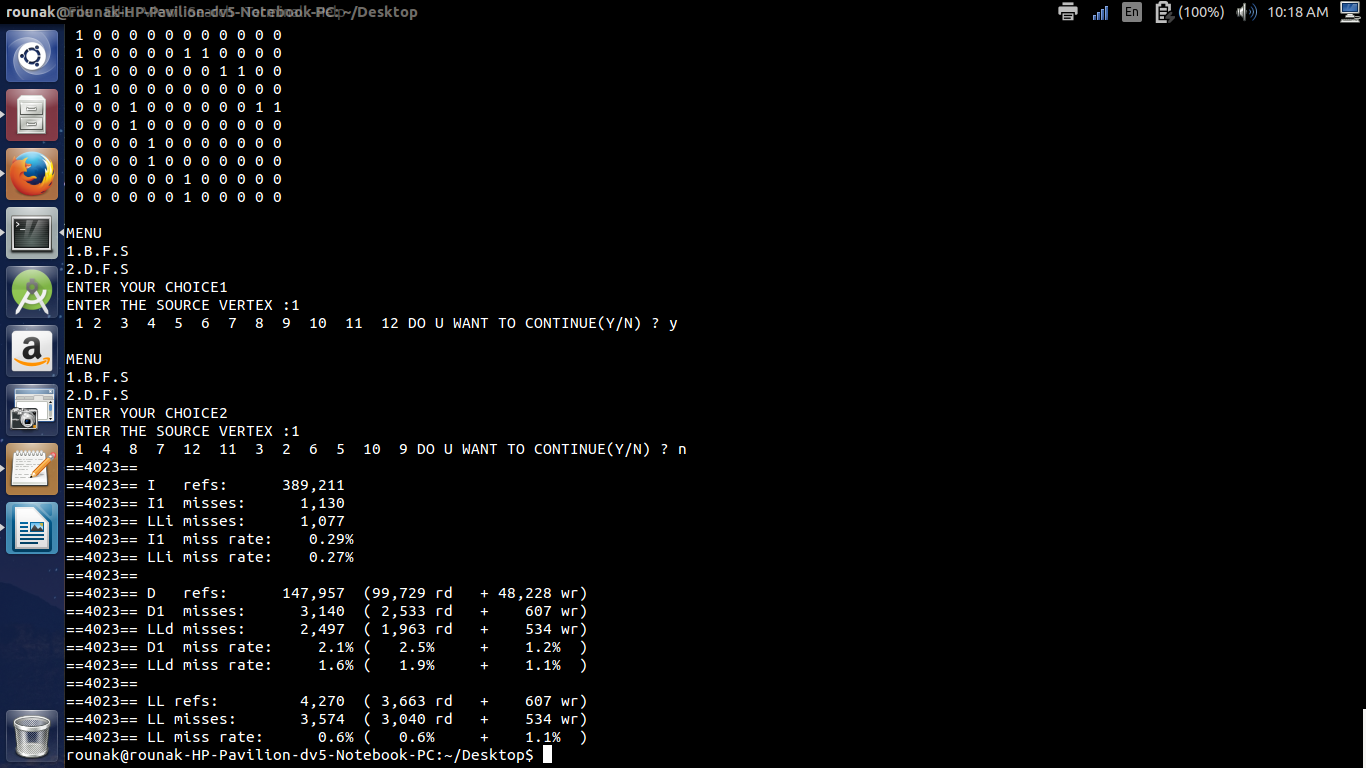
\includegraphics[width = 16cm]{project_1}
\caption{Cache Misses}
\end{figure}

\begin{figure}[h!]
\center
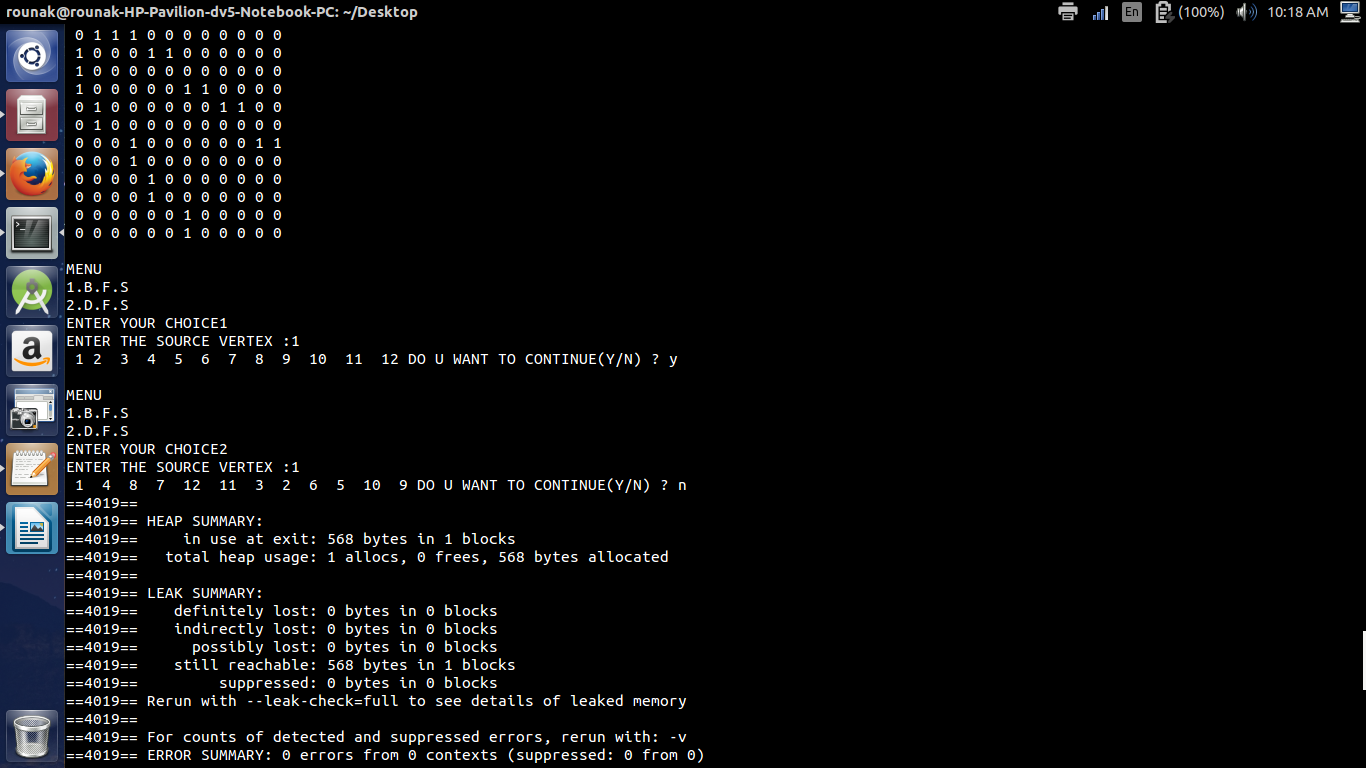
\includegraphics[width = 16cm]{project_2}
\caption{Memory Leaks}
\end{figure}

\begin{figure}[h!]
\center
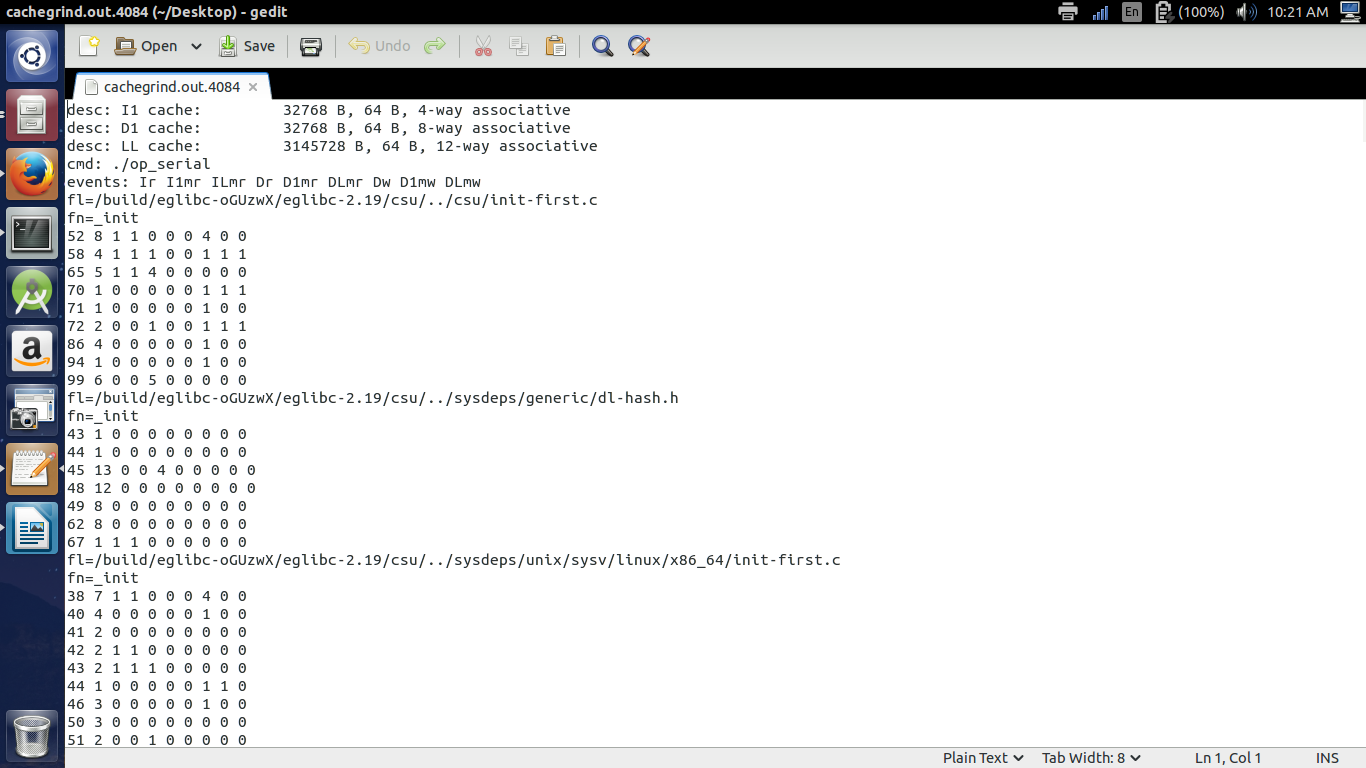
\includegraphics[width = 16cm]{project_4}
\caption{Annotated}
\end{figure}

\begin{figure}[h!]
\center
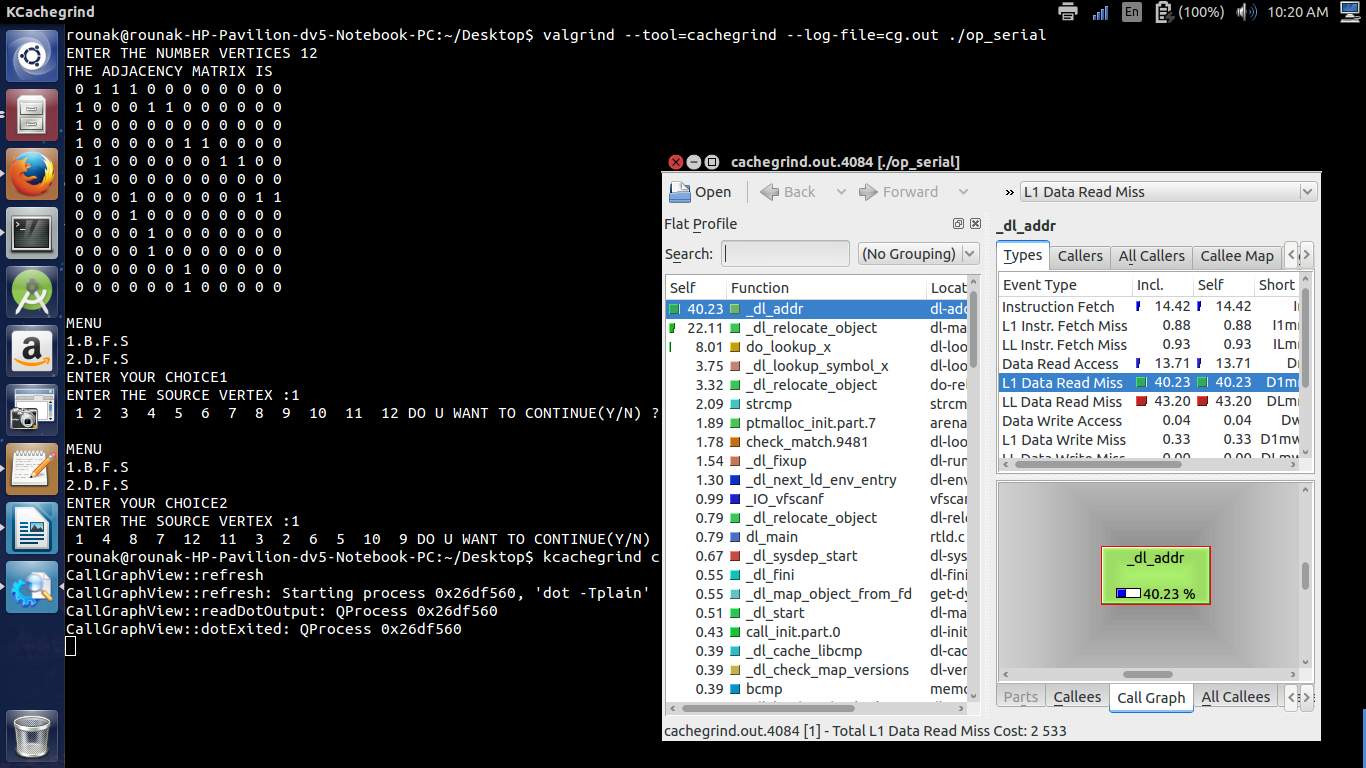
\includegraphics[width = 16cm]{project_3}
\caption{Kcachegrind-1}
\end{figure}

\begin{figure}[h!]
\center
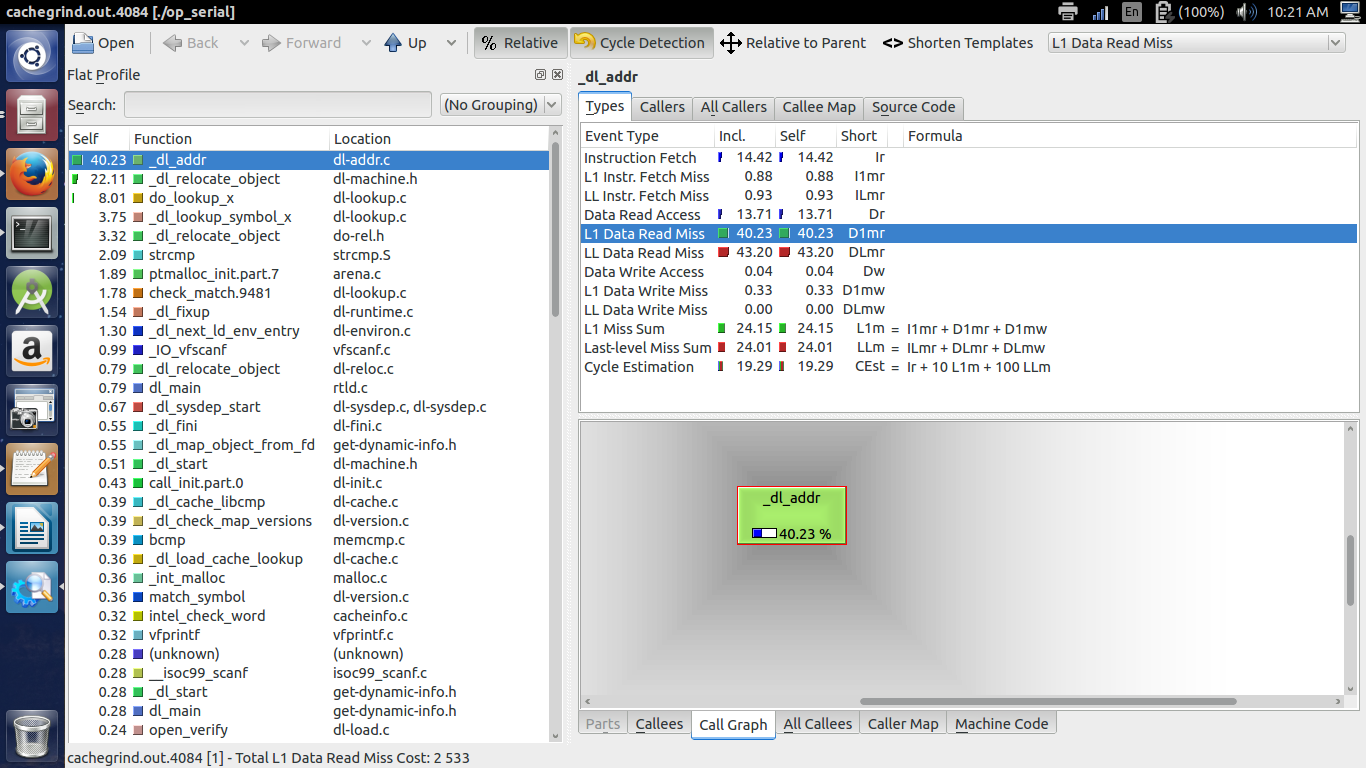
\includegraphics[width = 16cm]{project_5}
\caption{Kcachegrind-2}
\end{figure}



\end{document}
